\section{Модель нагрева слоя ПММА при экспонировании}

При экспонировании образца в нем происходит выделение энергии, что приводит к дополнительному нагреву. Поскольку в методе СЭЛТР температура резиста непосредственным образом определяет интенсивность различных процессов, влияющих на конечный профиль линии, необходимо оценить масштаб этого явления.

Моделирование нагрева образца проводилось на основе подхода, описанного в разделе~\ref{sec:sim_heating}, для следующих условий экспонирования: экспонирование ``в~кадр'', размеры кадра составляли 2.4$\times$1.9 мм$\pp$, ток экспонирования -- 5 нА, энергия электронного пучка -- 20 кэВ, толщина слоя ПММА -- 900 нм, число линий в кадре -- 625, расстояние между линиями -- 3 мкм, время экспонирования -- 100 с, температура образца -- 130~$^\circ$C.
Для вычисления интегралов в формуле~\ref{eq:heat_final_equation} использовался метод Монте-Карло, что позволило достичь компромисса между временем, необходимым для вычислений, и точностью вычислений.

Моделирование нагрева образца при экспонировании показало, что увеличение температуры ПММА в центре линии составляет менее 1~$^\circ$C (рисунок~\ref{fig:heating}). Это позволило в дальнейшем считать, что при экспонировании ``в кадр'' при характерных размерах области экспонирования порядка нескольких миллиметров и токе экспонирования в диапазоне 1-10 нА повышением температуры ПММА можно пренебречь.

\begin{figure}[h]
	\begin{center}
		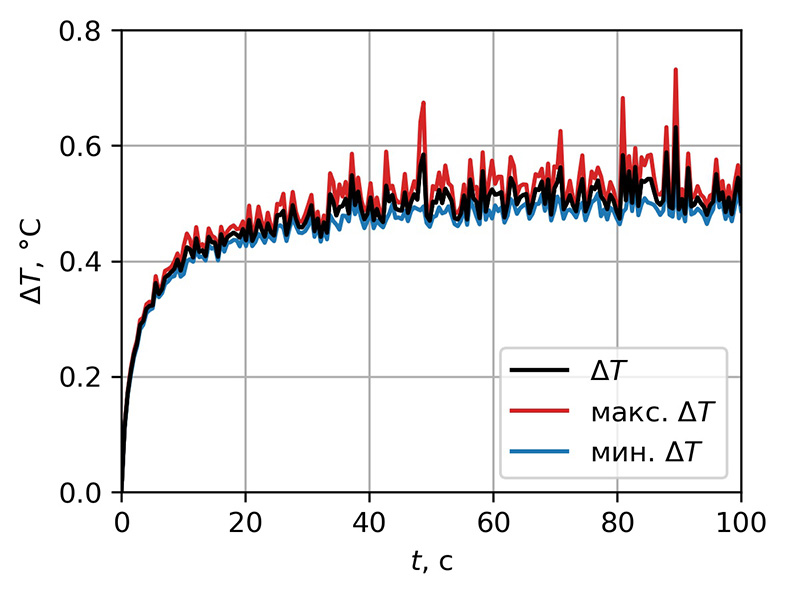
\includegraphics[width=0.6\linewidth]{heating/heating_200.jpg}
	\end{center}
	\vspace{-1em}
	\caption{Промоделированное увеличение температуры ПММА в центре линии на глубине, равной половине толщины слоя ПММА, при экспонировании ``в кадр'' с размерами кадра 2.4$\times$1.9 мм$\pp$. Ток экспонирования -- 5 нА, энергия электронного пучка -- 20 кэВ, толщина слоя ПММА -- 900 нм, число линий в кадре -- 625, расстояние между линиями -- 3~мкм, время экспонирования -- 100 с, температура образца -- 130~$^\circ$C. Наличие минимального и максимального значений $\Delta T$ обусловлено использованием метода Монте-Карло для вычисления интегралов в формуле~\ref{eq:heat_final_equation}.}
	\label{fig:heating}
\end{figure}




